If the input filename is of the form of one of the following \verb"<file>.in, <file>.inp, <file>.input" then the output filenames will take on the form be \verb"<file>_<type>.<ext>".
If the input file has any other extension, then the entire filename will simply be considered \verb"<file>" and similarly use the convetion \verb"<file>_<type>.<ext>" for each of the output files.

\section{Output Summary File}

OpenNodal generates a summary output file for the run results.
The naming convention for this summary file is \verb"<file>_results.out".
This file contains the final eigenvalue on the first line, followed by the final flux core averaged ratio of $\phi_2/\phi_1$ iff the problem was a 2 group problem.
The summary file will then have \verb"G" blocks giving the assembly averaged flux for each energy group mapped in a manner matching \verb"assm_map".

\section{Log File}

OpenNodal generates a log file echoing all output which is also printed to the screen, including any warnings or errors.
The naming convention for this summary file is \verb"<file>.log".

\section{Flux Output Files}

OpenNodal generates \verb"G" flux output files as well as a fission power output file.
The naming convention for these files is \verb"<file>_flux_g<g>.csv" and \verb"<file>_power.csv".
The data is listed in the following format:
\begin{verbatim}
x_centroid_node_row_1 y_centroid_node_col_1 flux_{g,1,1}
x_centroid_node_row_1 y_centroid_node_col_2 flux_{g,1,2}
x_centroid_node_row_1 y_centroid_node_col_3 flux_{g,1,3}
        :
x_centroid_node_row_1 y_centroid_node_col_Ny flux_{g,1,Ny}

x_centroid_node_row_2 y_centroid_node_col_1 flux_{g,2,1}
x_centroid_node_row_2 y_centroid_node_col_2 flux_{g,2,2}
        :
\end{verbatim}
So that it is a map for the node averaged flux of each group onto the centroid of the node to which it belongs.
Notice that each change in rows is separated by a blank line.
The power output is similar, except that the flux is replaced by node averaged power.
Note that since OpenNodal solves an eigenvalue problem, values should not be considered absolute but relative to each other.

\section{Flux Output Plots}

If the user has \verb"gnuplot" installed, then OpenNodal will generate plots of the groupwise flux, as well as the fission power.
The naming convention for these files is \verb"<file>_flux_g<g>.png" and \verb"<file>_power.png".
The files themselves are 2D heat-maps for the magnitude of the relative flux/power in each node across the whole core.
Example for the \verb"2d_ss_iaea-BSS11.inp" case with \verb"nsplit 64":
\begin{figure}[H]
\centering
  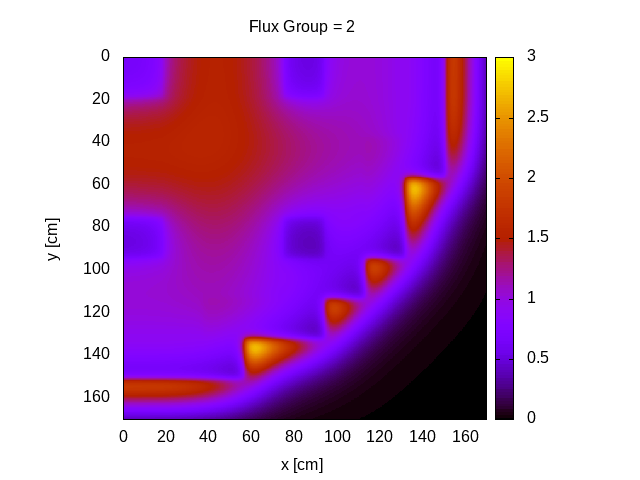
\includegraphics[width=0.7\textwidth]{chapters/output_form/images/2d_ss_iaea-BSS11_flux_g2.png}
  \caption{Thermal Flux for the BSS-11 Problem}
\end{figure}